% !TEX root = ./problem.en.tex
\gdef\thisproblemauthor{}
\gdef\thisproblemdeveloper{}
\gdef\thisproblemorigin{}
\begin{problem}{磨樹 Woody}
{standard input}{standard output}
{0.5 seconds}{512 MB}{}

Woody 是一位有著美學堅持的伐木工 \newline
他擁有一座森林,裡面的樹木都擁有方形樹幹 ( 如此完美!) \newline
他每天都會進行一次將樹幹磨得更細的工程 \newline
對於每棵樹選取接近根部的一小段樹幹,依圖中方式磨細 \newline
\newline
更精確地說,每次取橫切面 ( 正方形 ) 的中點連線 \newline
形成成較小的,旋轉 45 度的方形 \newline
再將這個小方形以外的部分磨掉 \newline
\newline
已之樹幹在截面積 $ \leq A $ 時會倒掉 \newline
給定一棵樹在第 0 天時的寬度 $ L $ \newline
Woody 從第 1 天開始磨樹 \newline
求這顆樹在第幾天會於磨樹途中或恰結束時倒掉 \newline

\centerline{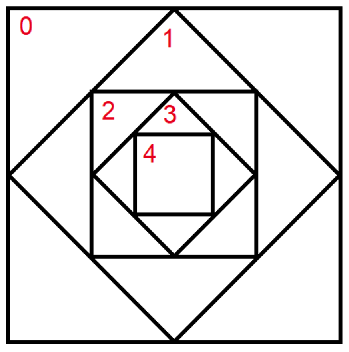
\includegraphics[scale=0.8]{./pics/A.png}}

\InputFile

輸入 2 個正整數 $ A $, $ L $ \newline
用空白分隔
\begin{iofmt}
\begin{itemize}
	\item $ A \leq 10^8 $
	\item $ L \leq 10^4 $
\end{itemize}
\end{iofmt}

\OutputFile

輸出一個整數,表示第幾天倒下

\Examples

\begin{example}
\exmpfile{./sample/PA-01.in.txt}{./sample/PA-01.out.txt}%
\exmpfile{./sample/PA-02.in.txt}{./sample/PA-02.out.txt}%
\exmpfile{./sample/PA-03.in.txt}{./sample/PA-03.out.txt}%
\end{example}

第一筆範例輸入,第0天截面積為 $1 \times 1 = 1$,直接倒下

\end{problem}
